\documentclass[12pt]{article}

\usepackage{helpers}

\begin{document}

Name: \makebox[3in]{\hrulefill
%NAME
\hrulefill}

\vfill

\begin{center}
{\huge Test 1}

{\large February 23, 2026}
\end{center}

\testrules

\vfill

\pledge

\newpage

\section*{Data Representation}

Please show your work.

%BEGIN_STANDARD_DR



\begin{enumerate}
\item Convert the unsigned binary integer 0b00011101 to decimal.
\vfill

\item Convert the unsigned binary integer 0b00011101 to hexadecimal.
\vfill


\item Convert the decimal number -22 to 8-bit two's complement binary.
\vfill

\item Convert the fixed point binary number 0b0100.1100 to decimal.
\vfill

\pagebreak
\item Subtract 0b01010001 - 0b01101111. These are two's complement binary numbers.
\vfill
\item Multiply 0b00001001 $\times$ 0b00001011. These are unsigned binary numbers.
\vfill
\item Write the string ``Um Ya Ya!'' as a sequence of ASCII values. An ASCII table is included at the end of this test.
\vfill
\end{enumerate}

\vfill

\standardsfooter

%END_STANDARD_DR

\newpage

\section*{Logic Representation}

Demonstrate understanding of boolean expressions and operations, logic circuits through computation and modeling.\\

%BEGIN_STANDARD_LR

\begin{enumerate}
\item Make a truth table for the boolean function $f(A,B,C) = (A\textrm{ xor }B)\textrm{ and }(\textrm{not }C)$.
\vfill

\item Draw a logic circuit for the function $f(A,B,C)$ from above.
\vfill

\pagebreak

\item Draw a logic circuit which triples a two-bit unsigned binary integer. There should be two input bits ($A$ and $B$) and four output bits ($C$, $D$, $E$, and $F$) such that $0\mathrm{b}AB \times 0\mathrm{b}11 = 0\mathrm{b}CDEF$. 

For example, $A=0$ and $B=1$ should give $C=0$, $D=0$, $E=1$, and $F=1$.

\vfill

\item Draw a logic circuit with two 1-bit inputs, $A$ and $B$. There should be one 1-bit output, $C$, which is what we get if we flip the bits of $A$ and $B$, and then multiply the flipped bits.

For example, if $A=1$ and $B=1$, the flipped bits would both be $0$, and their product would be $0$.

\vfill
\end{enumerate}

%END_STANDARD_LR

\vfill

\standardsfooter

\newpage

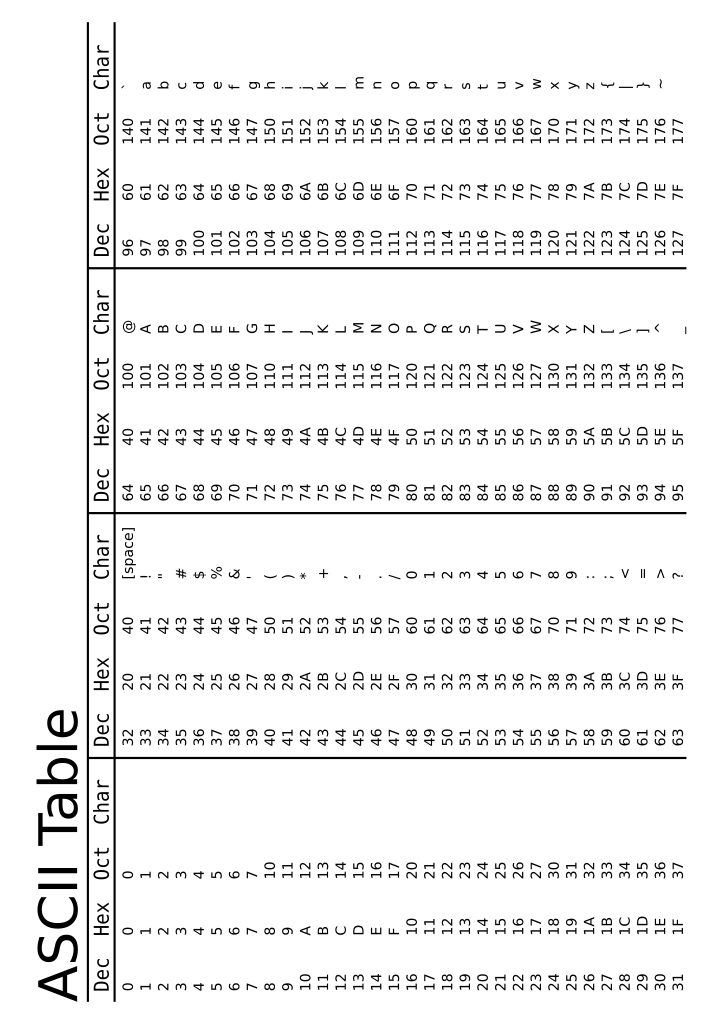
\includegraphics[height=\textheight]{wikimedia-ascii-table.png}

\end{document}